\textit{Before working with the data, a level of data pre-processing should be applied to ensure a workable dataset for the scene analysis and \gls{imu} based algorithm. This applies differently to the different data from Kaggle and is concerned with both formatting and cleaning the data.}

\section{Design Choices}
As mentioned in \textbf{\autoref{sec:data}}, we have decided to work with the dataset provided by Kaggle. This dataset contains four folders of data, where all the files within the file structure are regular text files (.txt). Since the purpose of each folder is different, as well as the file structure, different levels of formatting and cleaning is needed.

\begin{figure}[H]
    \centering
    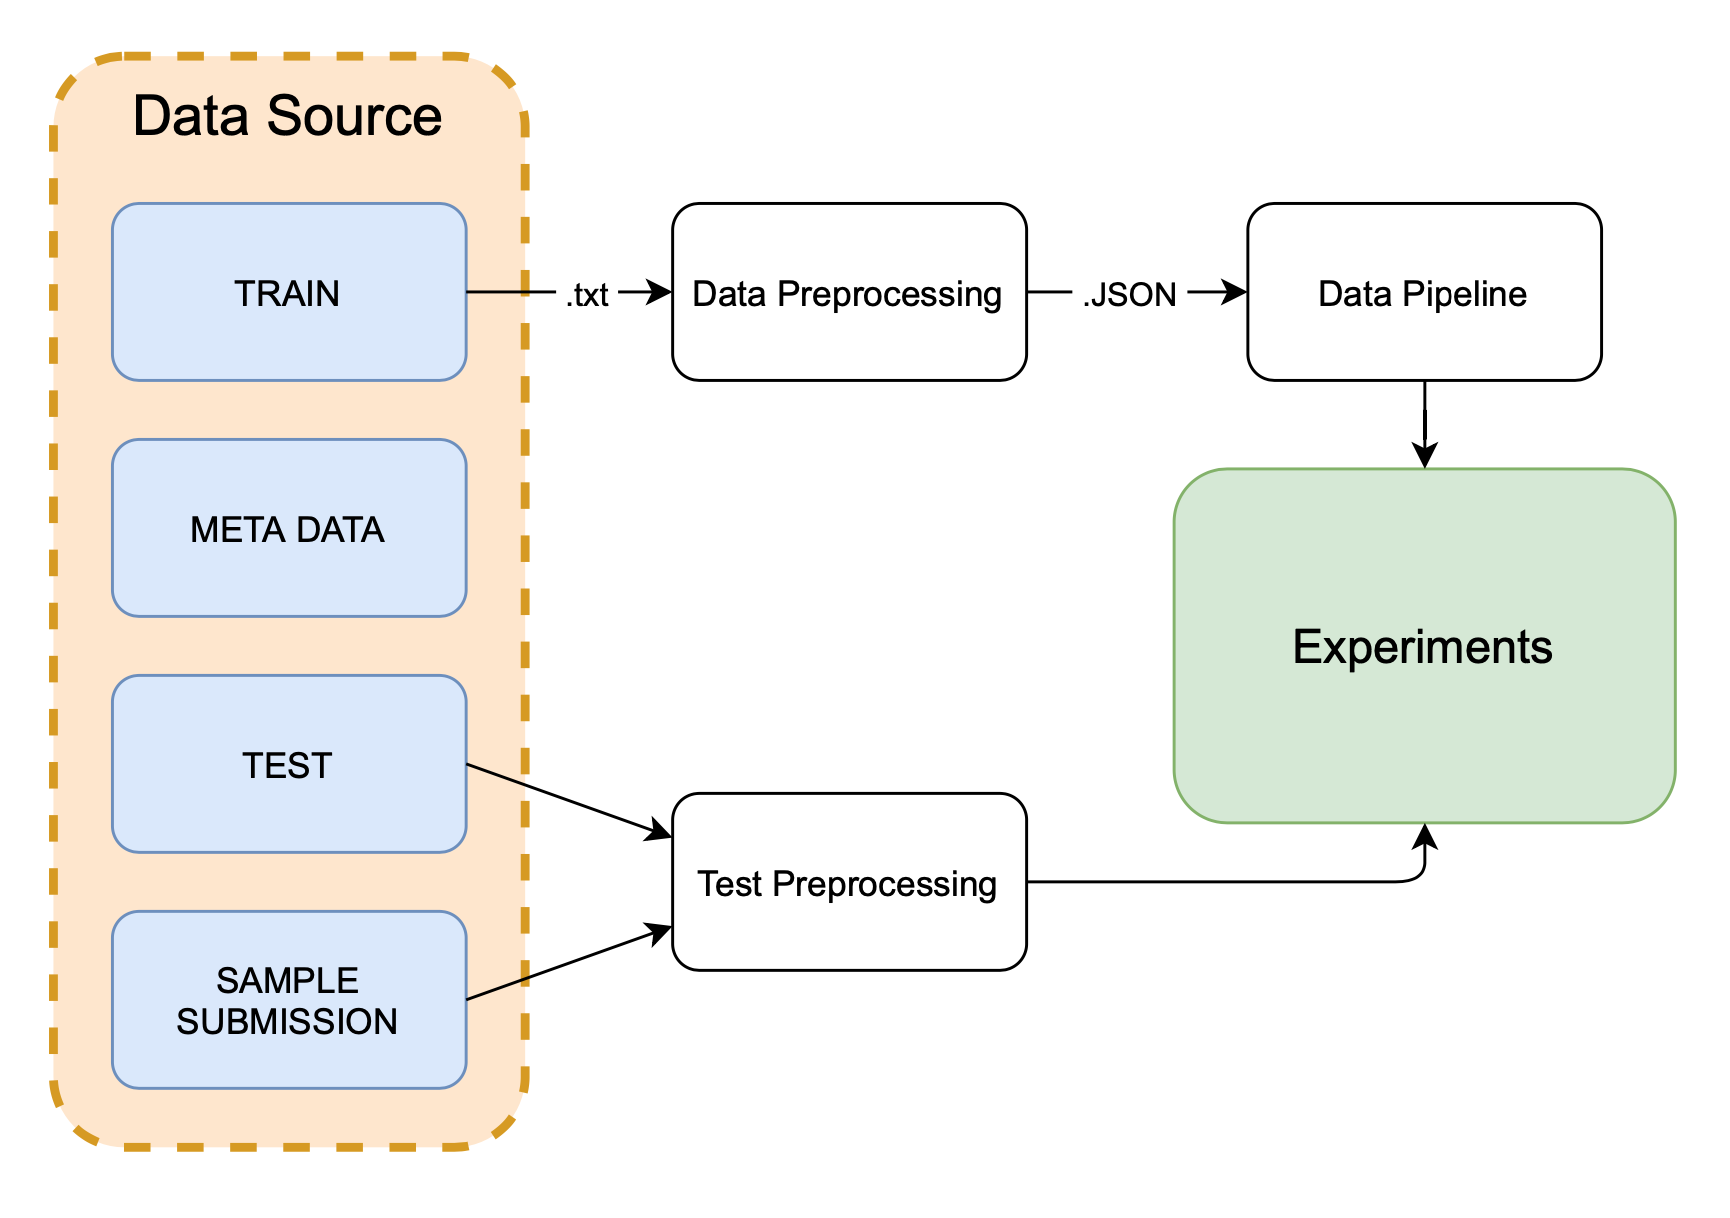
\includegraphics[scale=0.35]{Images/DataStandard/DataFlow.png}
    \caption{The overall architecture of data processing components}
    \label{fig:DataArchitecture}
\end{figure}

To determine how to prepare the data for scene analysis, we created an overall architecture of the data processing, which can be viewed on \textbf{\autoref{fig:DataArchitecture}}. The three different components, namely \textit{Data Preprocessing}, \textit{Data Pipeline} and \textit{Test Preprocessing} will be described in the following sections. The \textit{Data Preprocessing} will be divided into two parts: \textit{Train Data Conversion} and \textit{Train Data Cleaning}.

\subsection{Frameworks and Libraries}
%Python, pandas etc

\subsection{Train Data Conversion}
This process is a part of the \textit{Data Preprocessing} component depicted on \textbf{\autoref{fig:DataArchitecture}}. The first folder in the data source is the \textit{TRAIN} folder, which contains files on the regular text format, which we want to convert to \gls{json} format. The reason for this conversion is that \gls{json} is a universal data object format, supported by most languages by default or by adding a library. Additionally, we have chosen to remove the file structure, which first partitions the data into site and then floor level to instead simply add this information within each new \gls{json} file. This would result in \gls{json} files with a similar structure to \textbf{\autoref{fig:jsonformat}}.

\begin{figure}[H]
\lstset{numbers=left}
\begin{lstlisting}
{ 
    siteID:
    siteName:
    floorLevel:
    pathID:
    startTime:
    sensorData: 
        [
            {
                attributesFromKaggle
                label { x, y } // closest waypoint
            },
            {
                attributesFromKaggle
                label { x, y } // closest waypoint
            },
            ...
        ]
}
\end{lstlisting}
\caption{The \gls{json} format we have converted the data into.}
\label{fig:jsonformat}
\end{figure}

As seen on \textbf{\autoref{fig:jsonformat}}, each file contains information about which site (ID and name) and floor level the specific path has been measured at, alongside the ID of the path and a timestamp of when the measurement has begun. Lastly is an array containing the different sensor observations from the original path file. Each observation contains the original attributes, and we have determined and added the closest waypoint to each observation. The closest waypoint is determined by the timestamps meaning that the x- and y-coordinates for a sensor measurement are determined by the waypoint which is closest to the measurement. 

\subsection{Train Data Cleaning}
After processing the data to a new format, a level of data cleaning should also be enforced. This is concerned with normalising the floor level format to the same as the submission format. In the \gls{json} files the redundant data will be removed to minimise the size of each file. %Skal uddybes hvad er

%Problemet med new lines

%Outlier detection and removal such as looking whether the accelorometer values are proper.


\subsection{Data Pipeline} \label{sec:datapipeline}
After preprocessing, the data should be formatted after specific machine learning algorithms, which is depicted in \textbf{\autoref{fig:DataArchitecture}} as \textit{Data Pipeline}.

\subsection{Test Data Preprocessing}